\documentclass{article}
\usepackage{hyperref}
\usepackage{graphicx}
\usepackage[utf8]{inputenc}
\graphicspath{{./images/}}
\hypersetup{
    colorlinks=true,
    linkcolor=blue,
    filecolor=magenta,      
    urlcolor=cyan,
}
\urlstyle{same}
\title{ MAD1 - Analysis of a dataset about African Banking Crisis }
\date{ 03-01-2020 }
\author{ Fernando André Bezerra Moura Fernandes - bez0070@vsb.cz}

\begin{document}
    \maketitle
    \pagenumbering{gobble}
    \newpage
    \tableofcontents
    \newpage
    \pagenumbering{arabic}
    \section{ African Banking Crisis }
    
    A banking crisis reflects the crisis of liquidity and insolvency of one or more banks in 
    the financial system. Due to bank's sizable losses, bank encounters critical liquidity 
    shortage to the extent that this disrupts its ability in repaying the debt contracts and 
    the withdrawals demanded by depositors. 
    This dataset is a derivative of the Reinhart et. al's Global Financial Stability dataset.
    It is valuable to those who seek to understand the dynamics of financial stability within 
    the African context, since it focuses on the Banking, Debt, Financial, Inflation and Systemic
    Crises that occurred, from 1860 to 2014, in 13 African countries, including: Algeria, 
    Angola, Central African Republic, Ivory Coast, Egypt, Kenya, Mauritius, Morocco, Nigeria, 
    South Africa, Tunisia, Zambia and Zimbabwe.
    It was obtained using \textbf{Kaggle} at: \url{https://www.kaggle.com/chirin/africa-economic-banking-and-systemic-crisis-data}.
    This document will describe and explain the some correlations found analyzing the dataset. 
    \newpage
    \section{ Continuous Variable Analysis}
    The \textbf{USD Exchange Rate} is the amount of local country currency you could exchange for 1 
    american dollar (USD) and the \textbf{Annual CPI Inflation} is the change in the prices 
    of a basket of goods and services that are typically purchased by specific groups of 
    households measured by the \textbf{ Consumer Price Index(CPI) }. 
    The first measure allows us to verify the quality of the countries' currency 
    comparing it to a normally stable and strong one like the USD and the second
    measure is useful to see the changes of prices of products in the country. 
    
    \begin{figure}[h!]
        \caption{Standard Deviation of the Annual Cpi Inflation per country}
        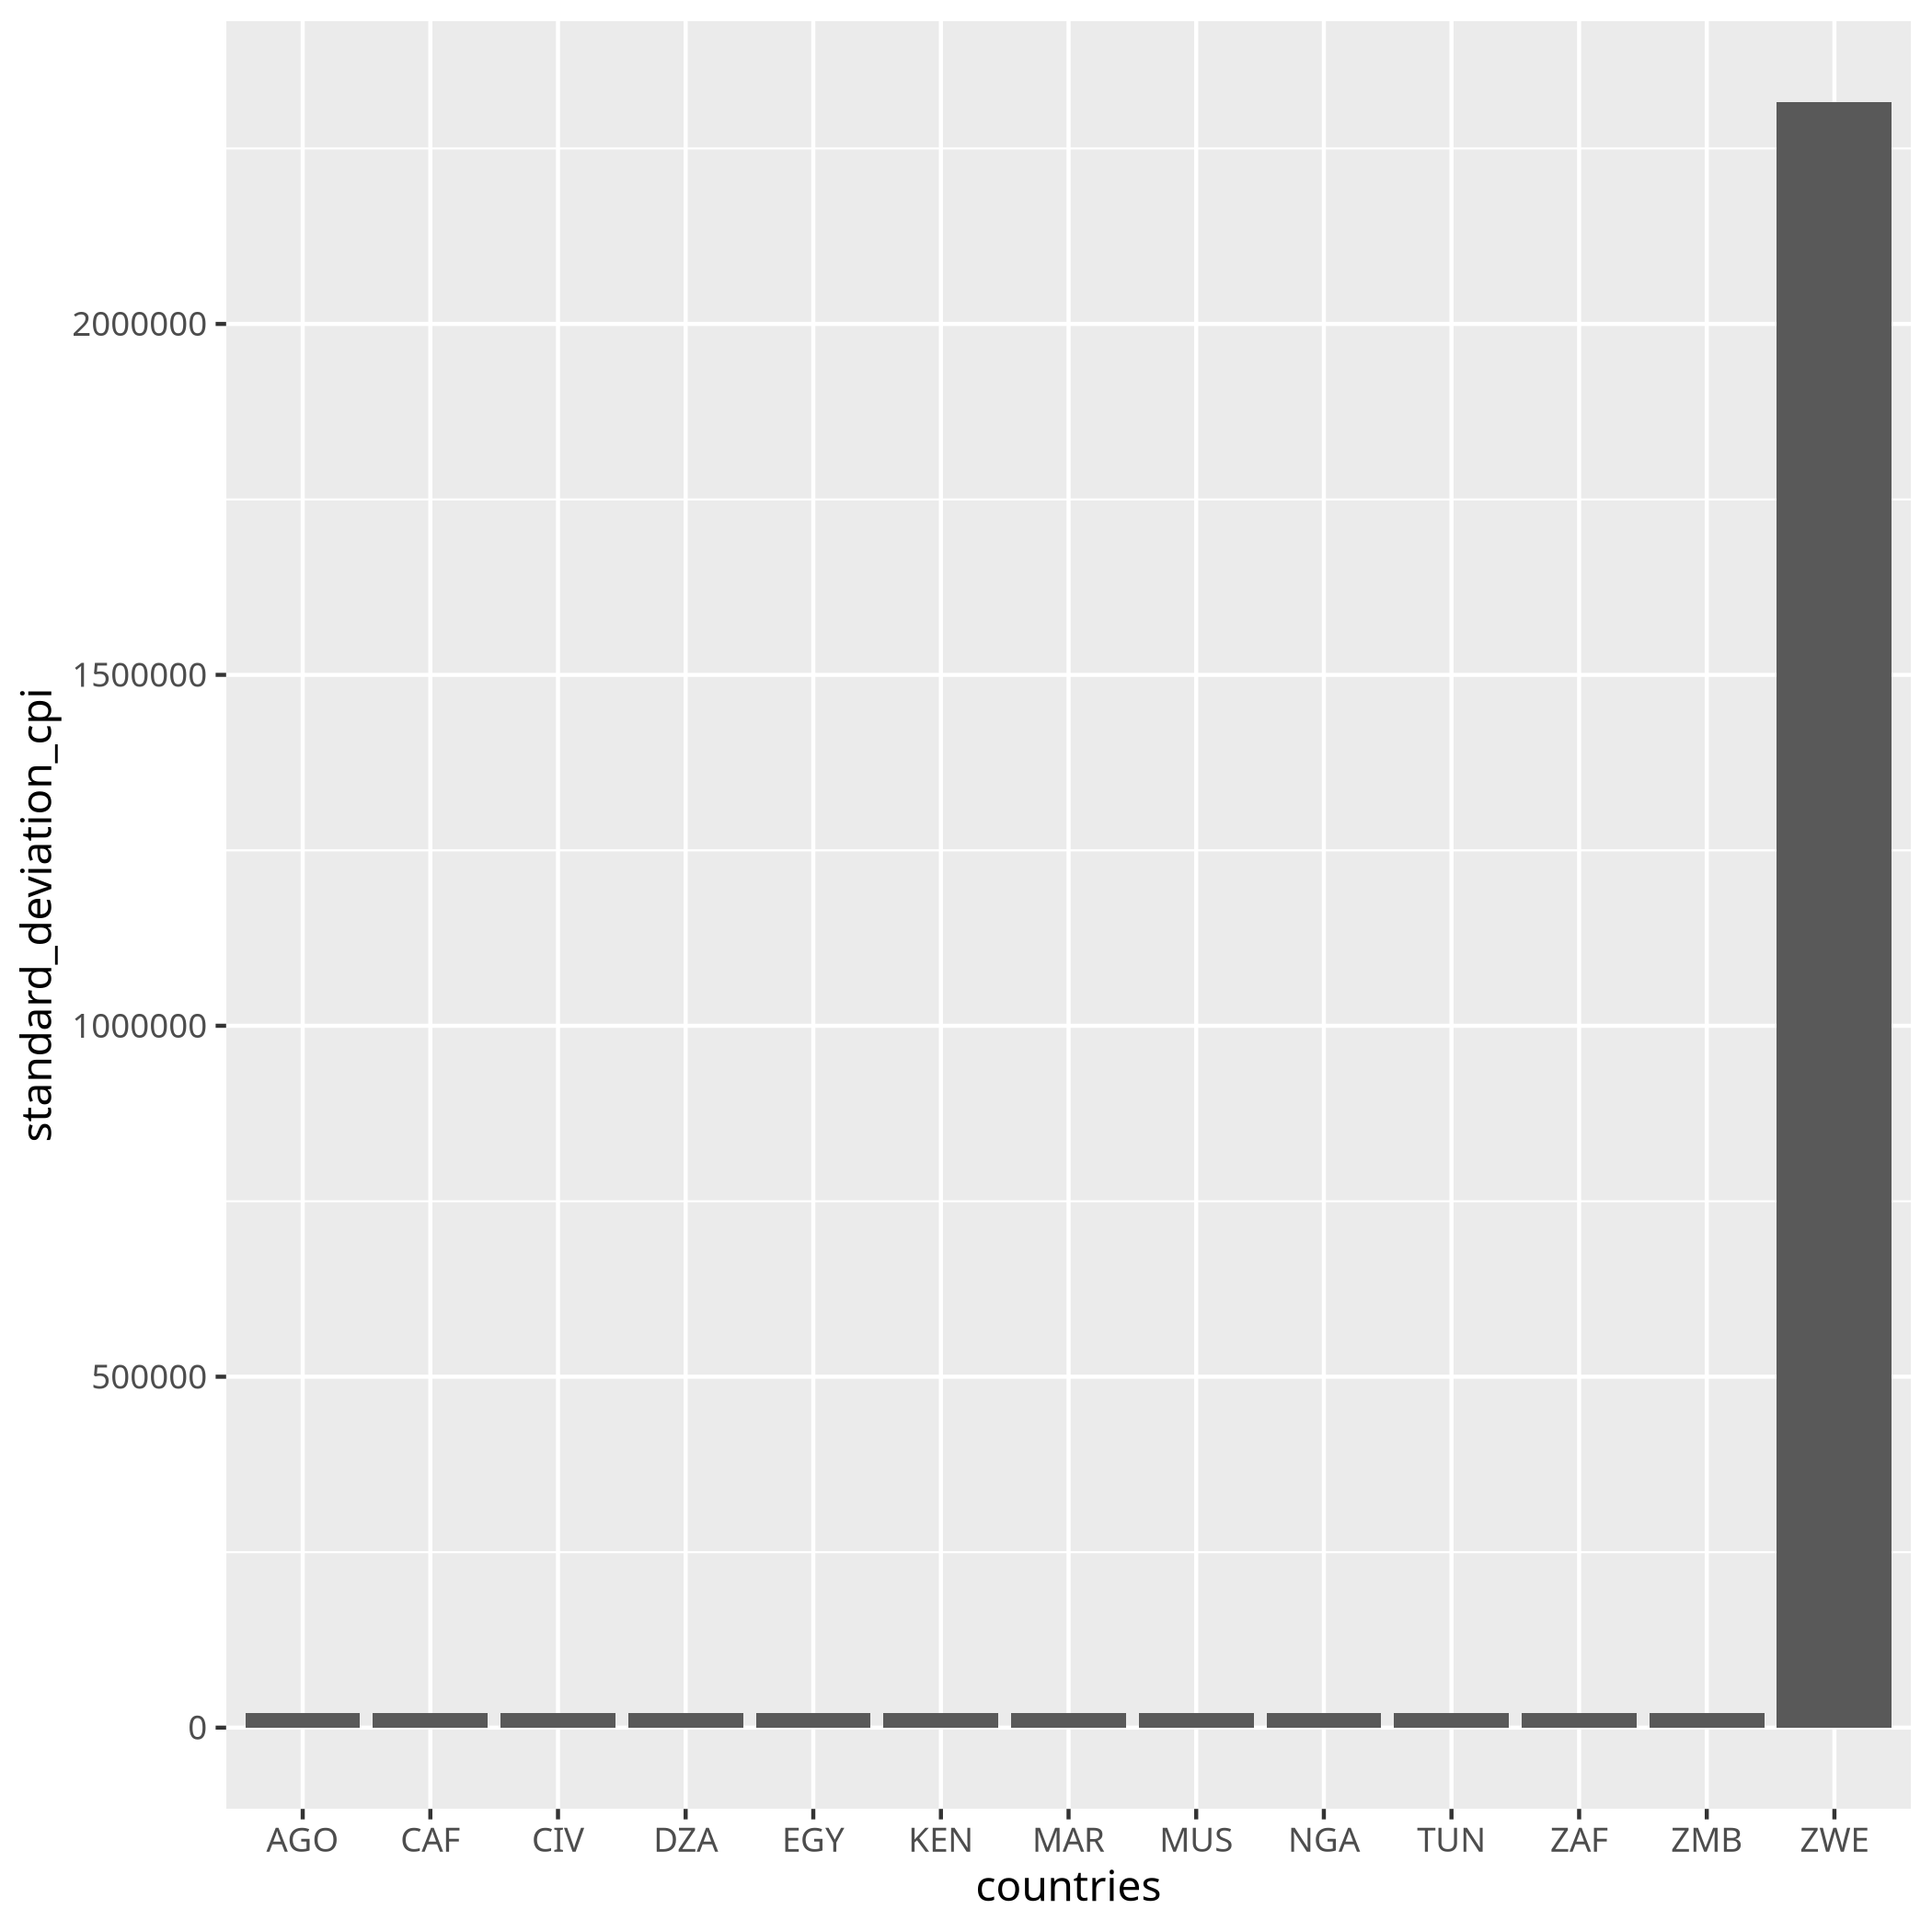
\includegraphics[scale=0.7]{plot4_cpi.png}
    \end{figure}
    \newpage
    \begin{figure}[h!]
        \caption{ Standard Deviation of the USD Exchange Rate per country}
        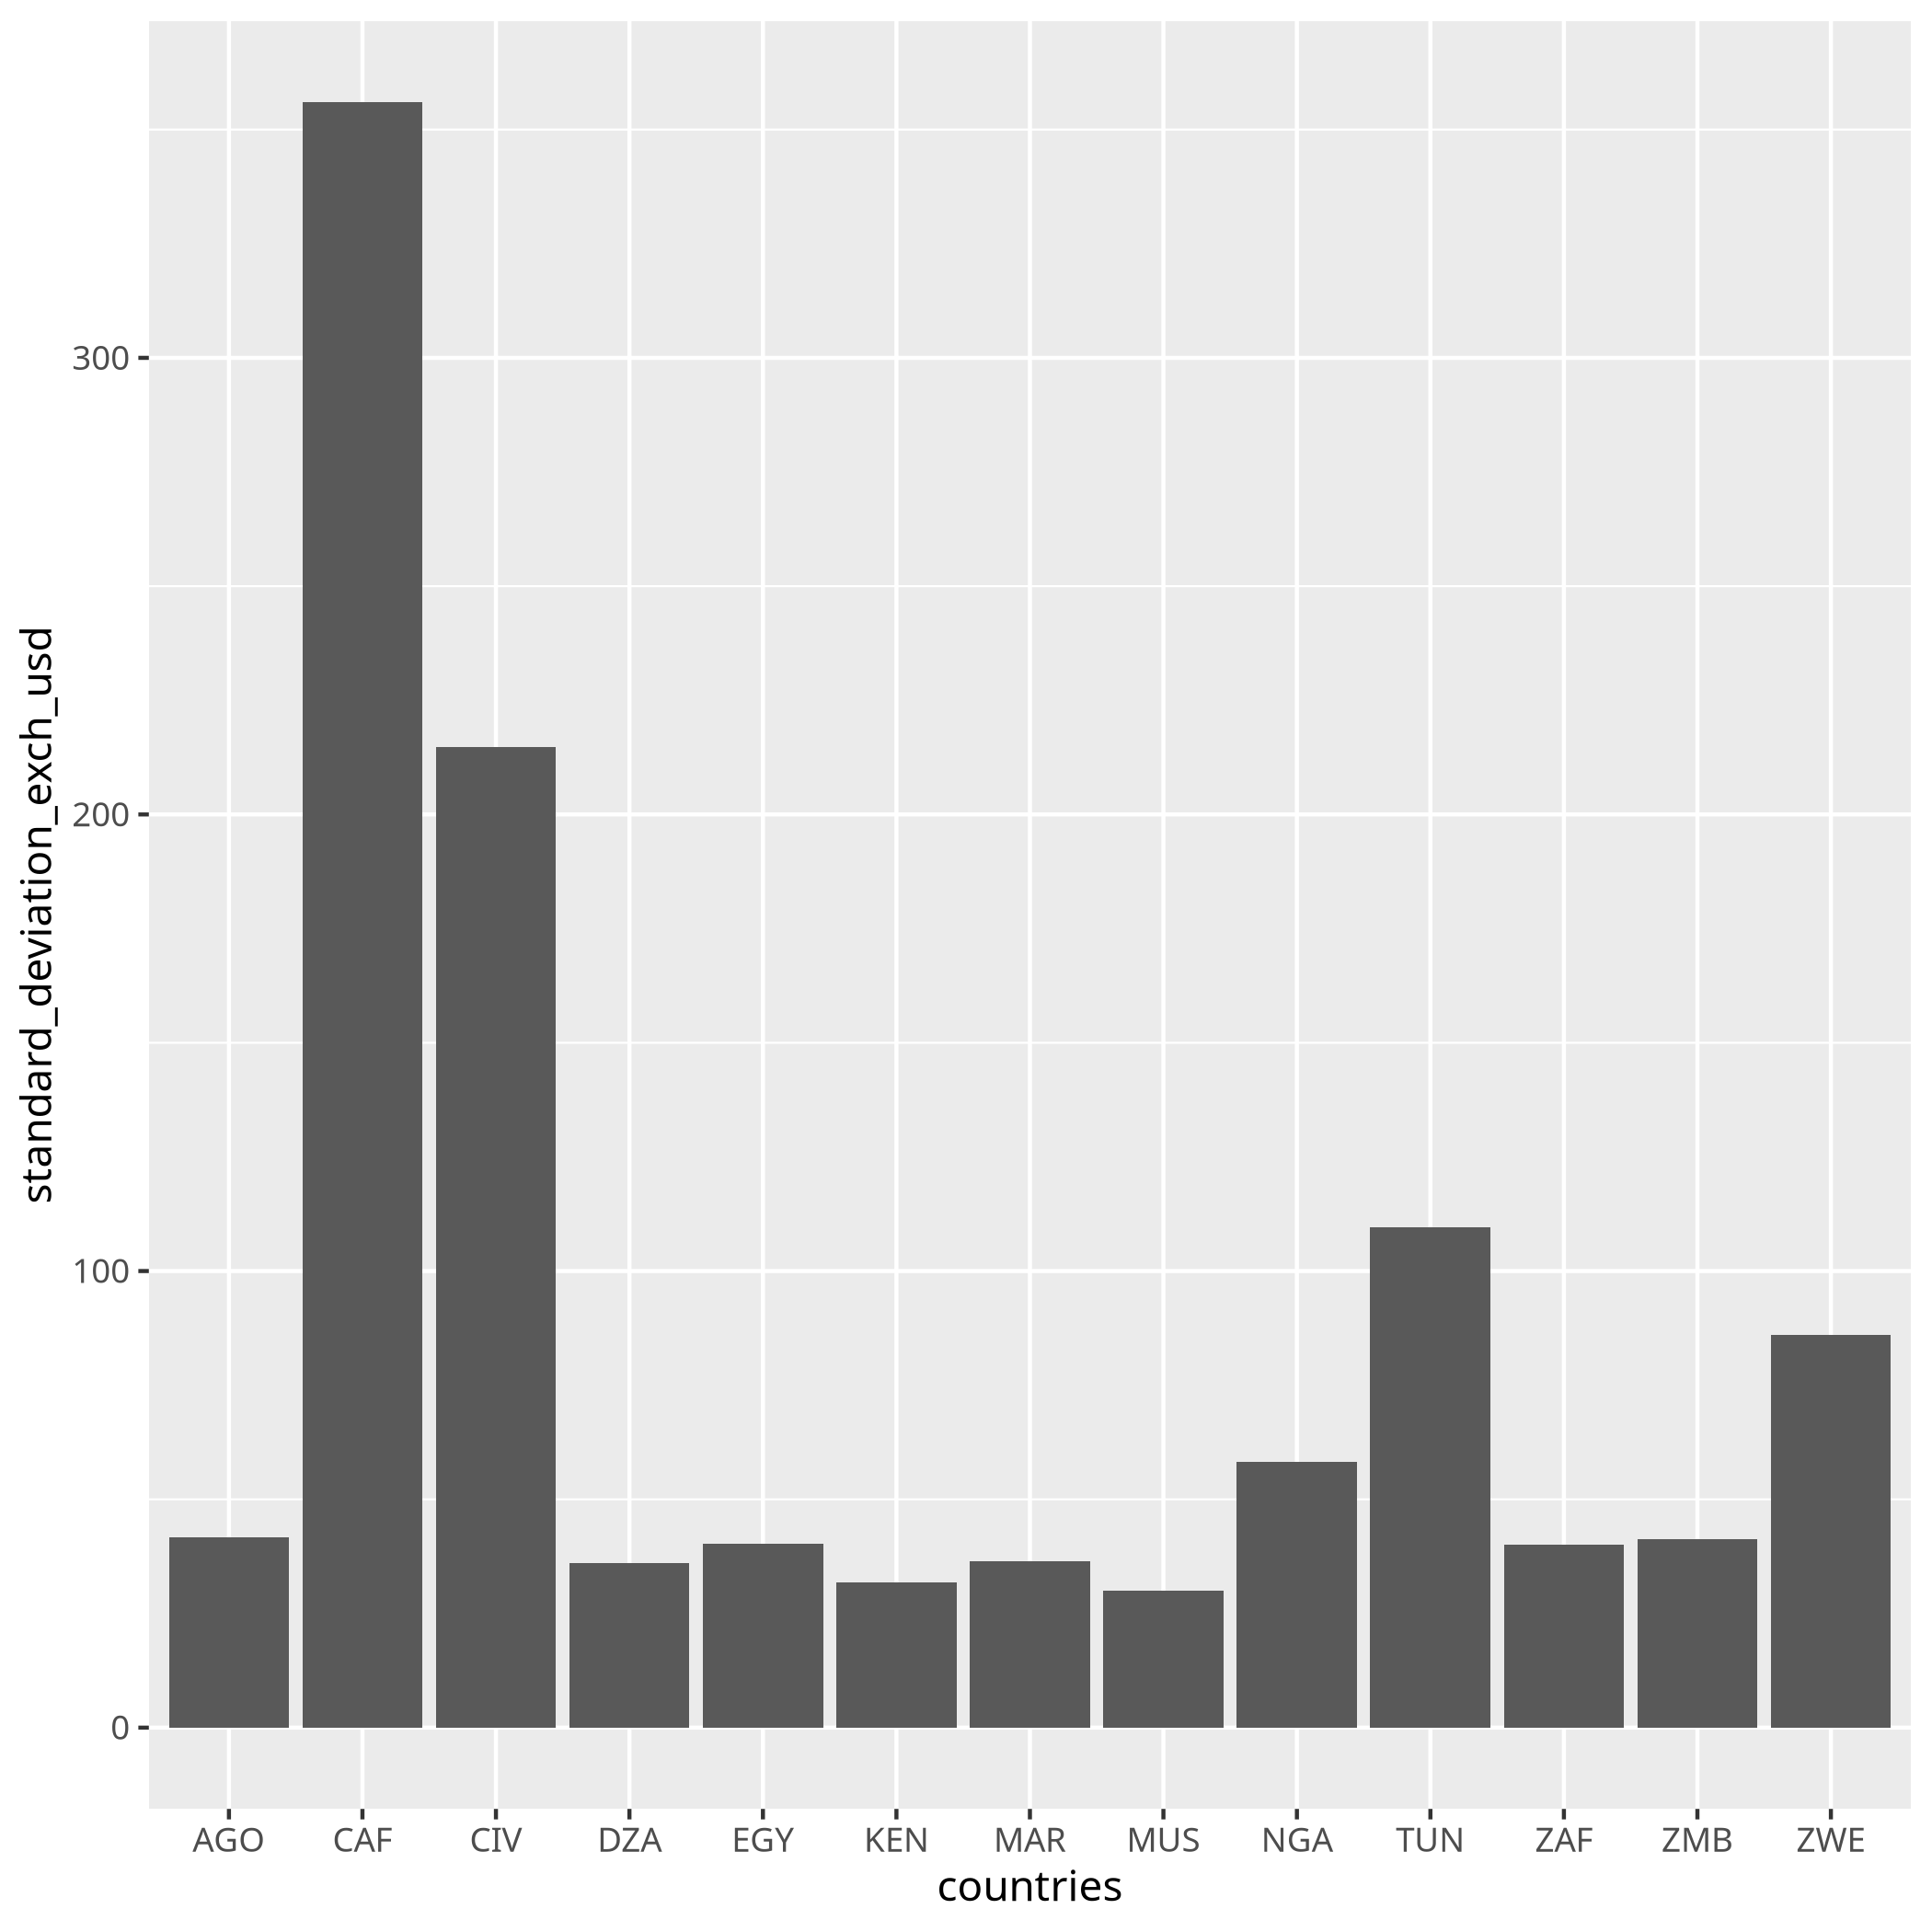
\includegraphics[scale=0.7]{plot4_exch_usd.png}
    \end{figure}
    
    
    The measured average Annual CPI Inflation of all the countries in the dataset is 
    \textbf{20848.89 \%}  and the average USD Exchange Rate is \textbf{43.14083}.
    According to Figure 1, \textbf{Zimbabwe} has an huge mean deviation from the 
    average Annual CPI Inflation, with a very big difference when taking into account 
    the rest of the countries. 
    If we calculate Zimbabwe's average Annual CPI Inflation we obtain a value of \textbf{245105.6 \%}, 
    which means that during the years, hyperinflation has affected the country more than any other 
    and can explain the destruction of the country's productive sector(agriculture i.e).
    By analyzing Figure 2 we can verify that the spotlight now goes to the 
    \textbf{Central African Republic}.
    By calculating its average USD Exchange Rate we obtain \textbf{367.6861} 
    which is a extremely higher than the ones from other countries on this dataset. 
    This can lead to the conclusion of the weakness of the currency that is used in this country, 
    the \textbf{Central African CFA Franc (XAF)}.

    \newpage
    \section{Systemic Crisis}
    A \textbf{Systemic Crisis} is a domino effect in which a financial trouble spreads
    between institutions and markets until it affects the whole monetary
    and financial system with dire global economic consequences.
    \begin{figure}[h!]
        \caption{ Systemic Crisis in all the countries along the years }
        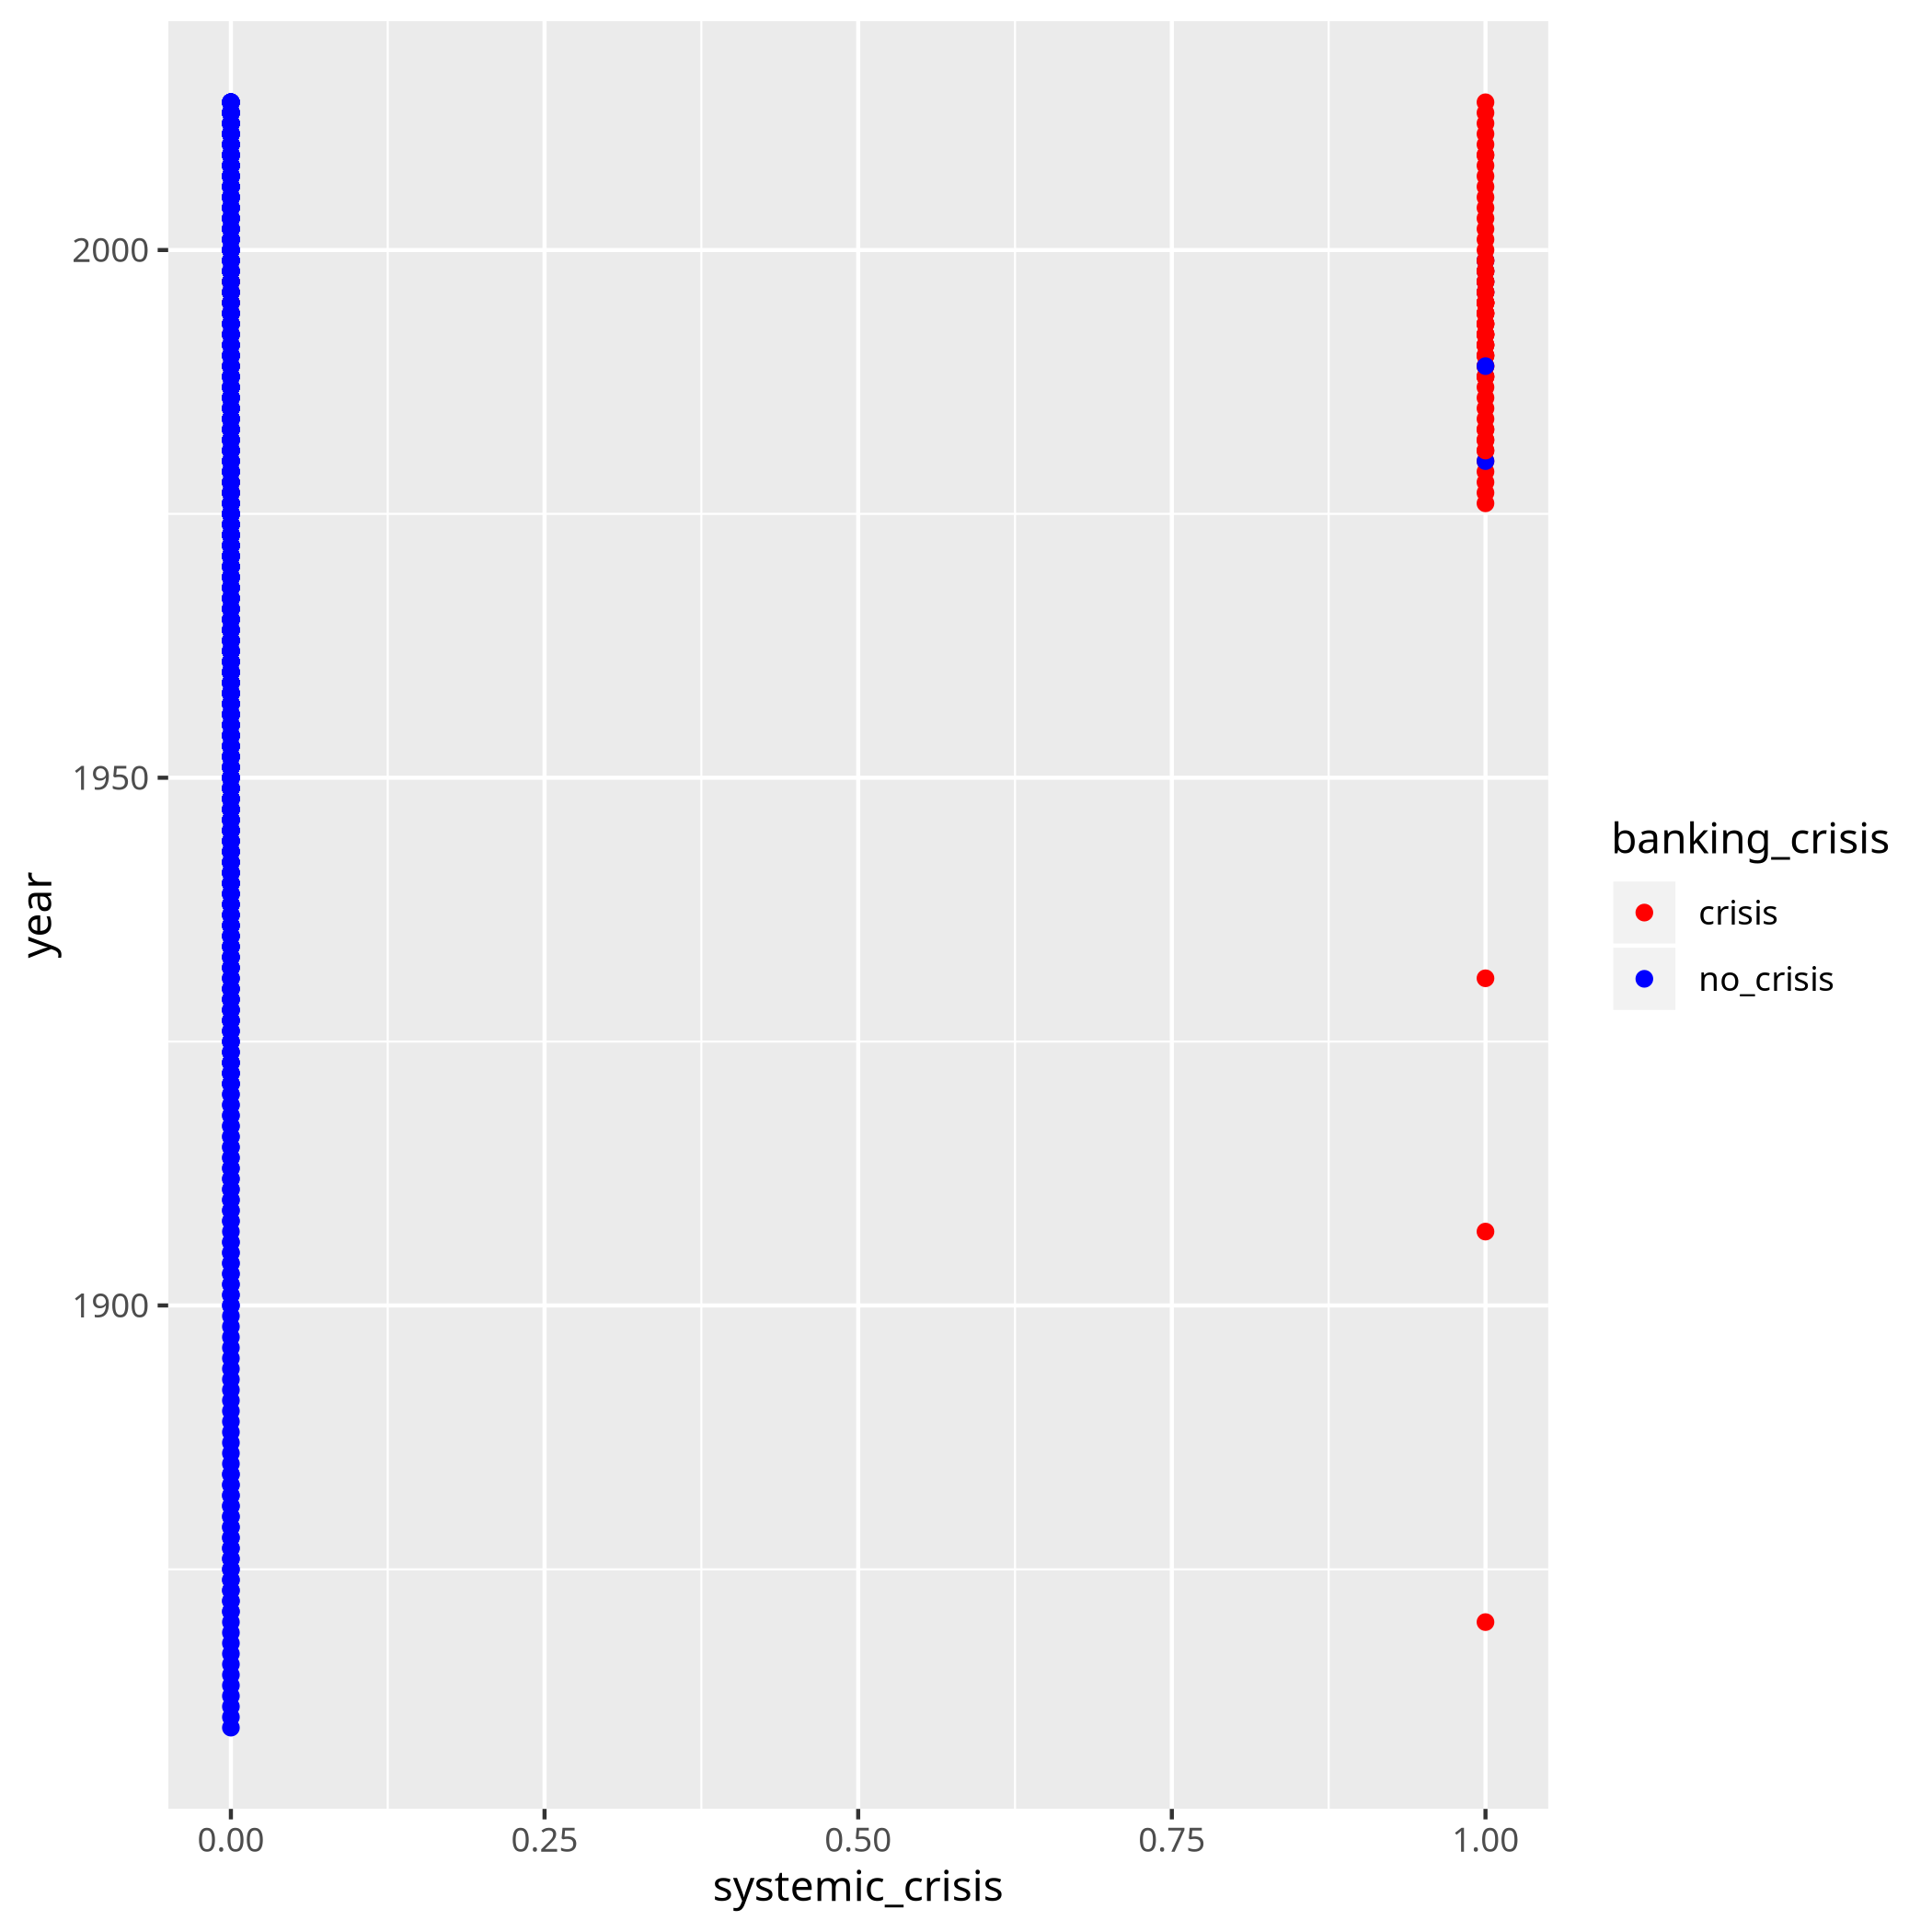
\includegraphics[scale=0.7]{plot1.png}
    \end{figure} 

    Looking at Figure 3, we can conclude that a financial trouble in a country's economy 
    easily spreads to the banking institutions, as debts need to be payed and 
    either by bank runs(where depositors widthraw huge amounts of money from their accounts 
    fearing bank failure) or by bank panics, it leads to shortage on bank money supply 
    and to a banking crisis.
    
    \newpage
    \section{Annual CPI Inflation}
    \subsection{ Banking Crisis }
    As already explained the Annual CPI Inflation helps us see a country's population purchasing 
    power.
    \begin{figure}[h!]
        \caption{ Annual CPI Inflation in relation with a banking crisis}
        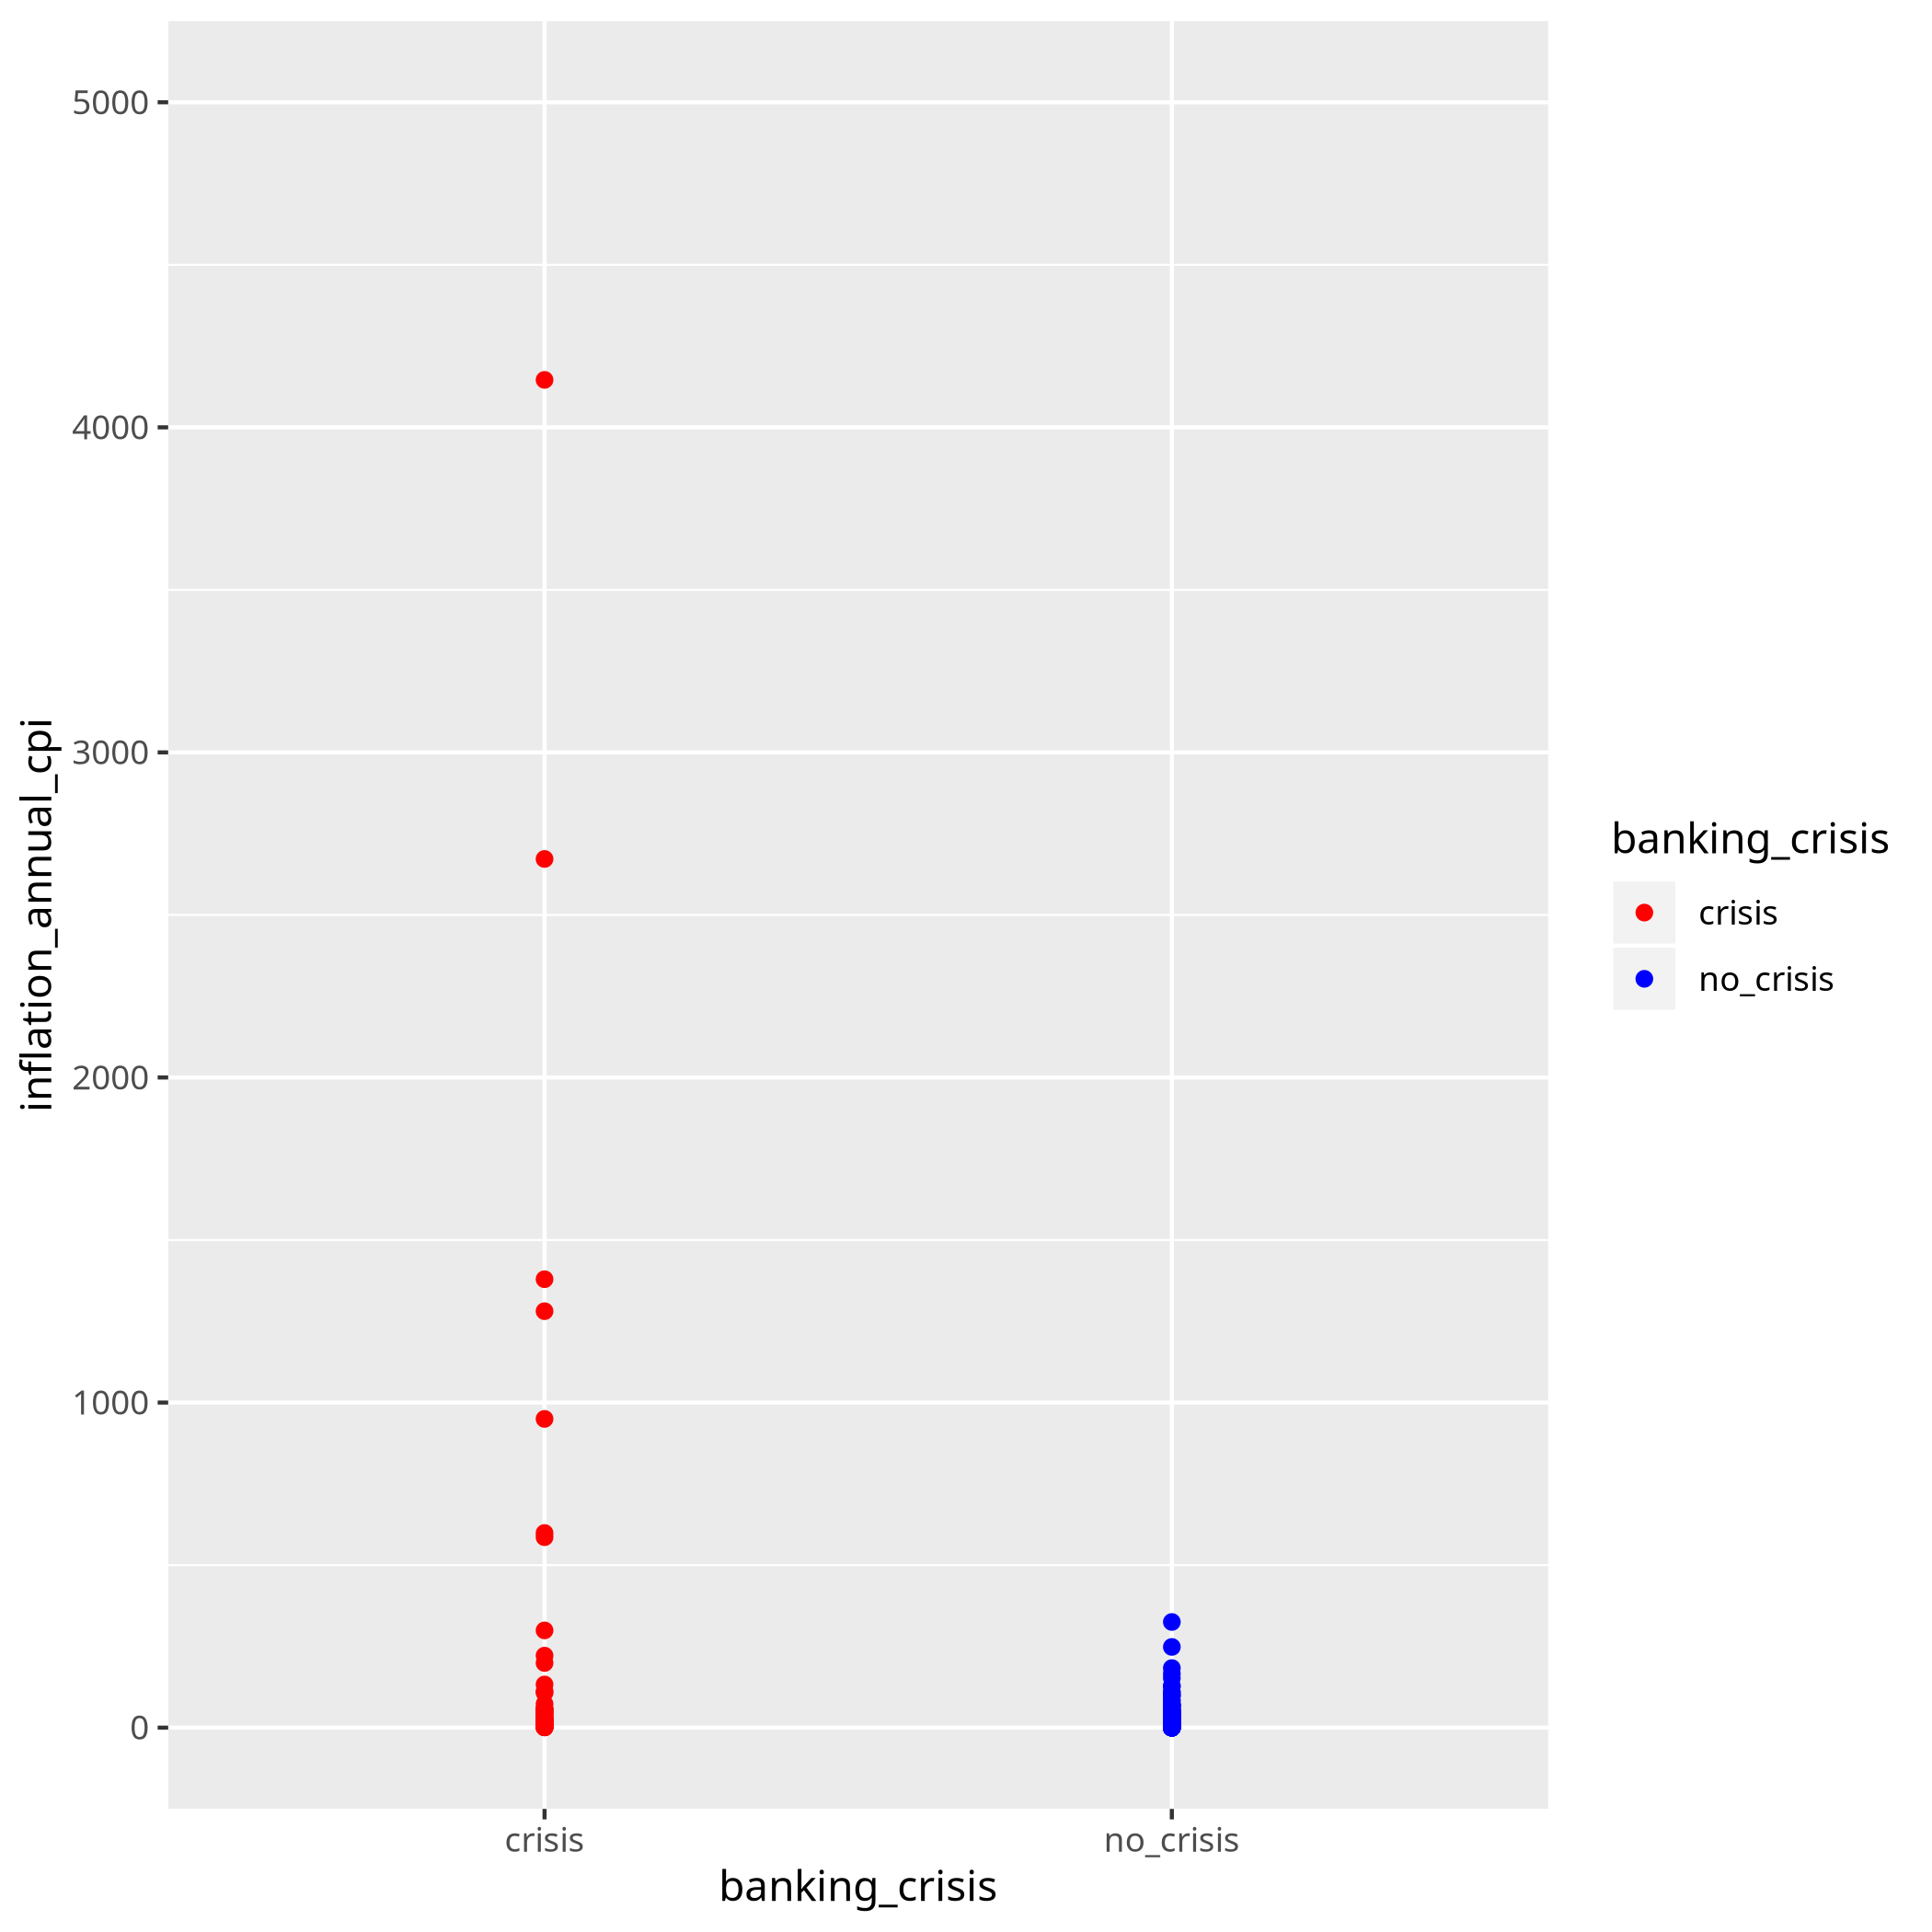
\includegraphics[scale=0.7]{plot2.png}
    \end{figure}
    
    By analyzing the 4th figure, we can see that after the 500\% Annual Inflation CPI threshold,
    it is practically certain that the country will face a banking crisis. This may be related 
    to the need of the everyday citizen needing more bank loans to fulfill their needs since
    the the prices are going up.
    
    \newpage
    \subsection{ Inflation Crisis }
    An \textbf{Inflation Crisis} occurs whenever \textbf{hyperinflation} occurs. 
    \textbf{Hyperinflation} is a very high and typically accelerating inflation. 
    It quickly erodes the real value of the local currency, 
    as the prices  of all goods increase. 
    This causes people to minimize their holdings in that currency as they usually 
    switch to more stable foreign currencies, often the US Dollar.

    \begin{figure}[h!]
        \caption{ CPI Inflation in relation with a crisis in inflation in Angola}
        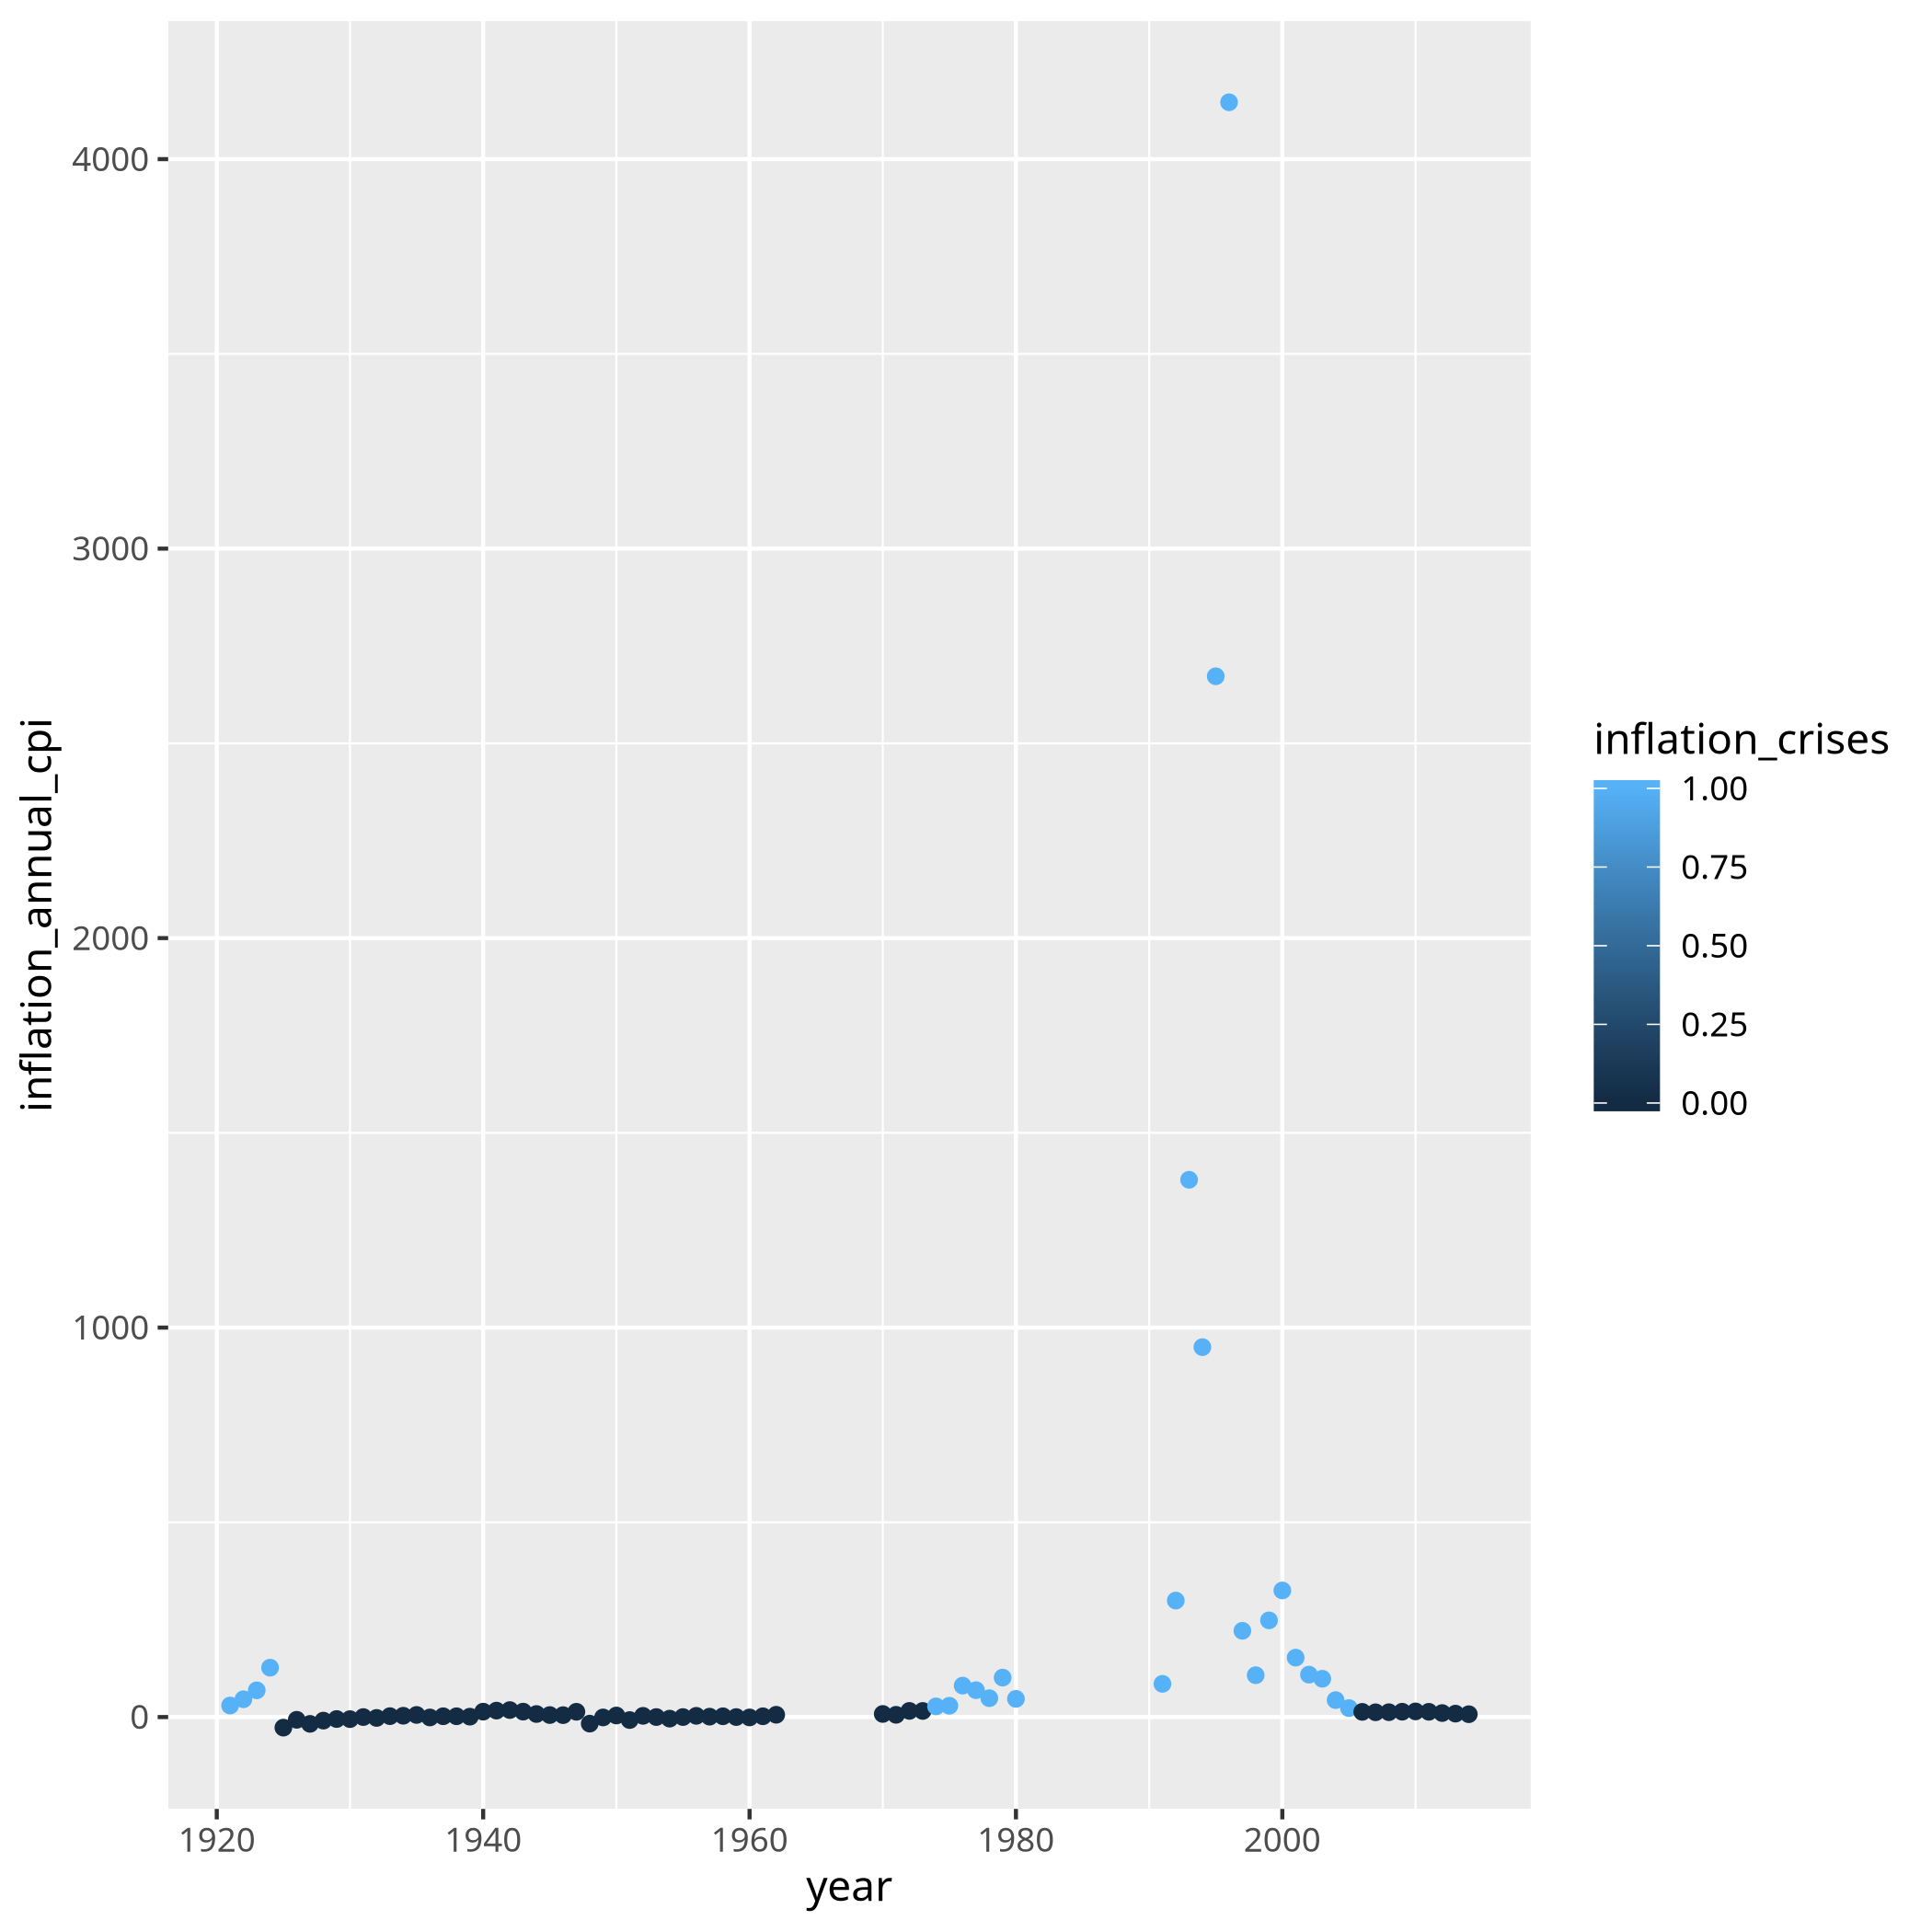
\includegraphics[scale=0.7]{plot3_angola.png}
    \end{figure}
    
    \newpage
    
    \begin{figure}[h!]
        \caption{ CPI Inflation in relation with a crisis in inflation in Zambia}
        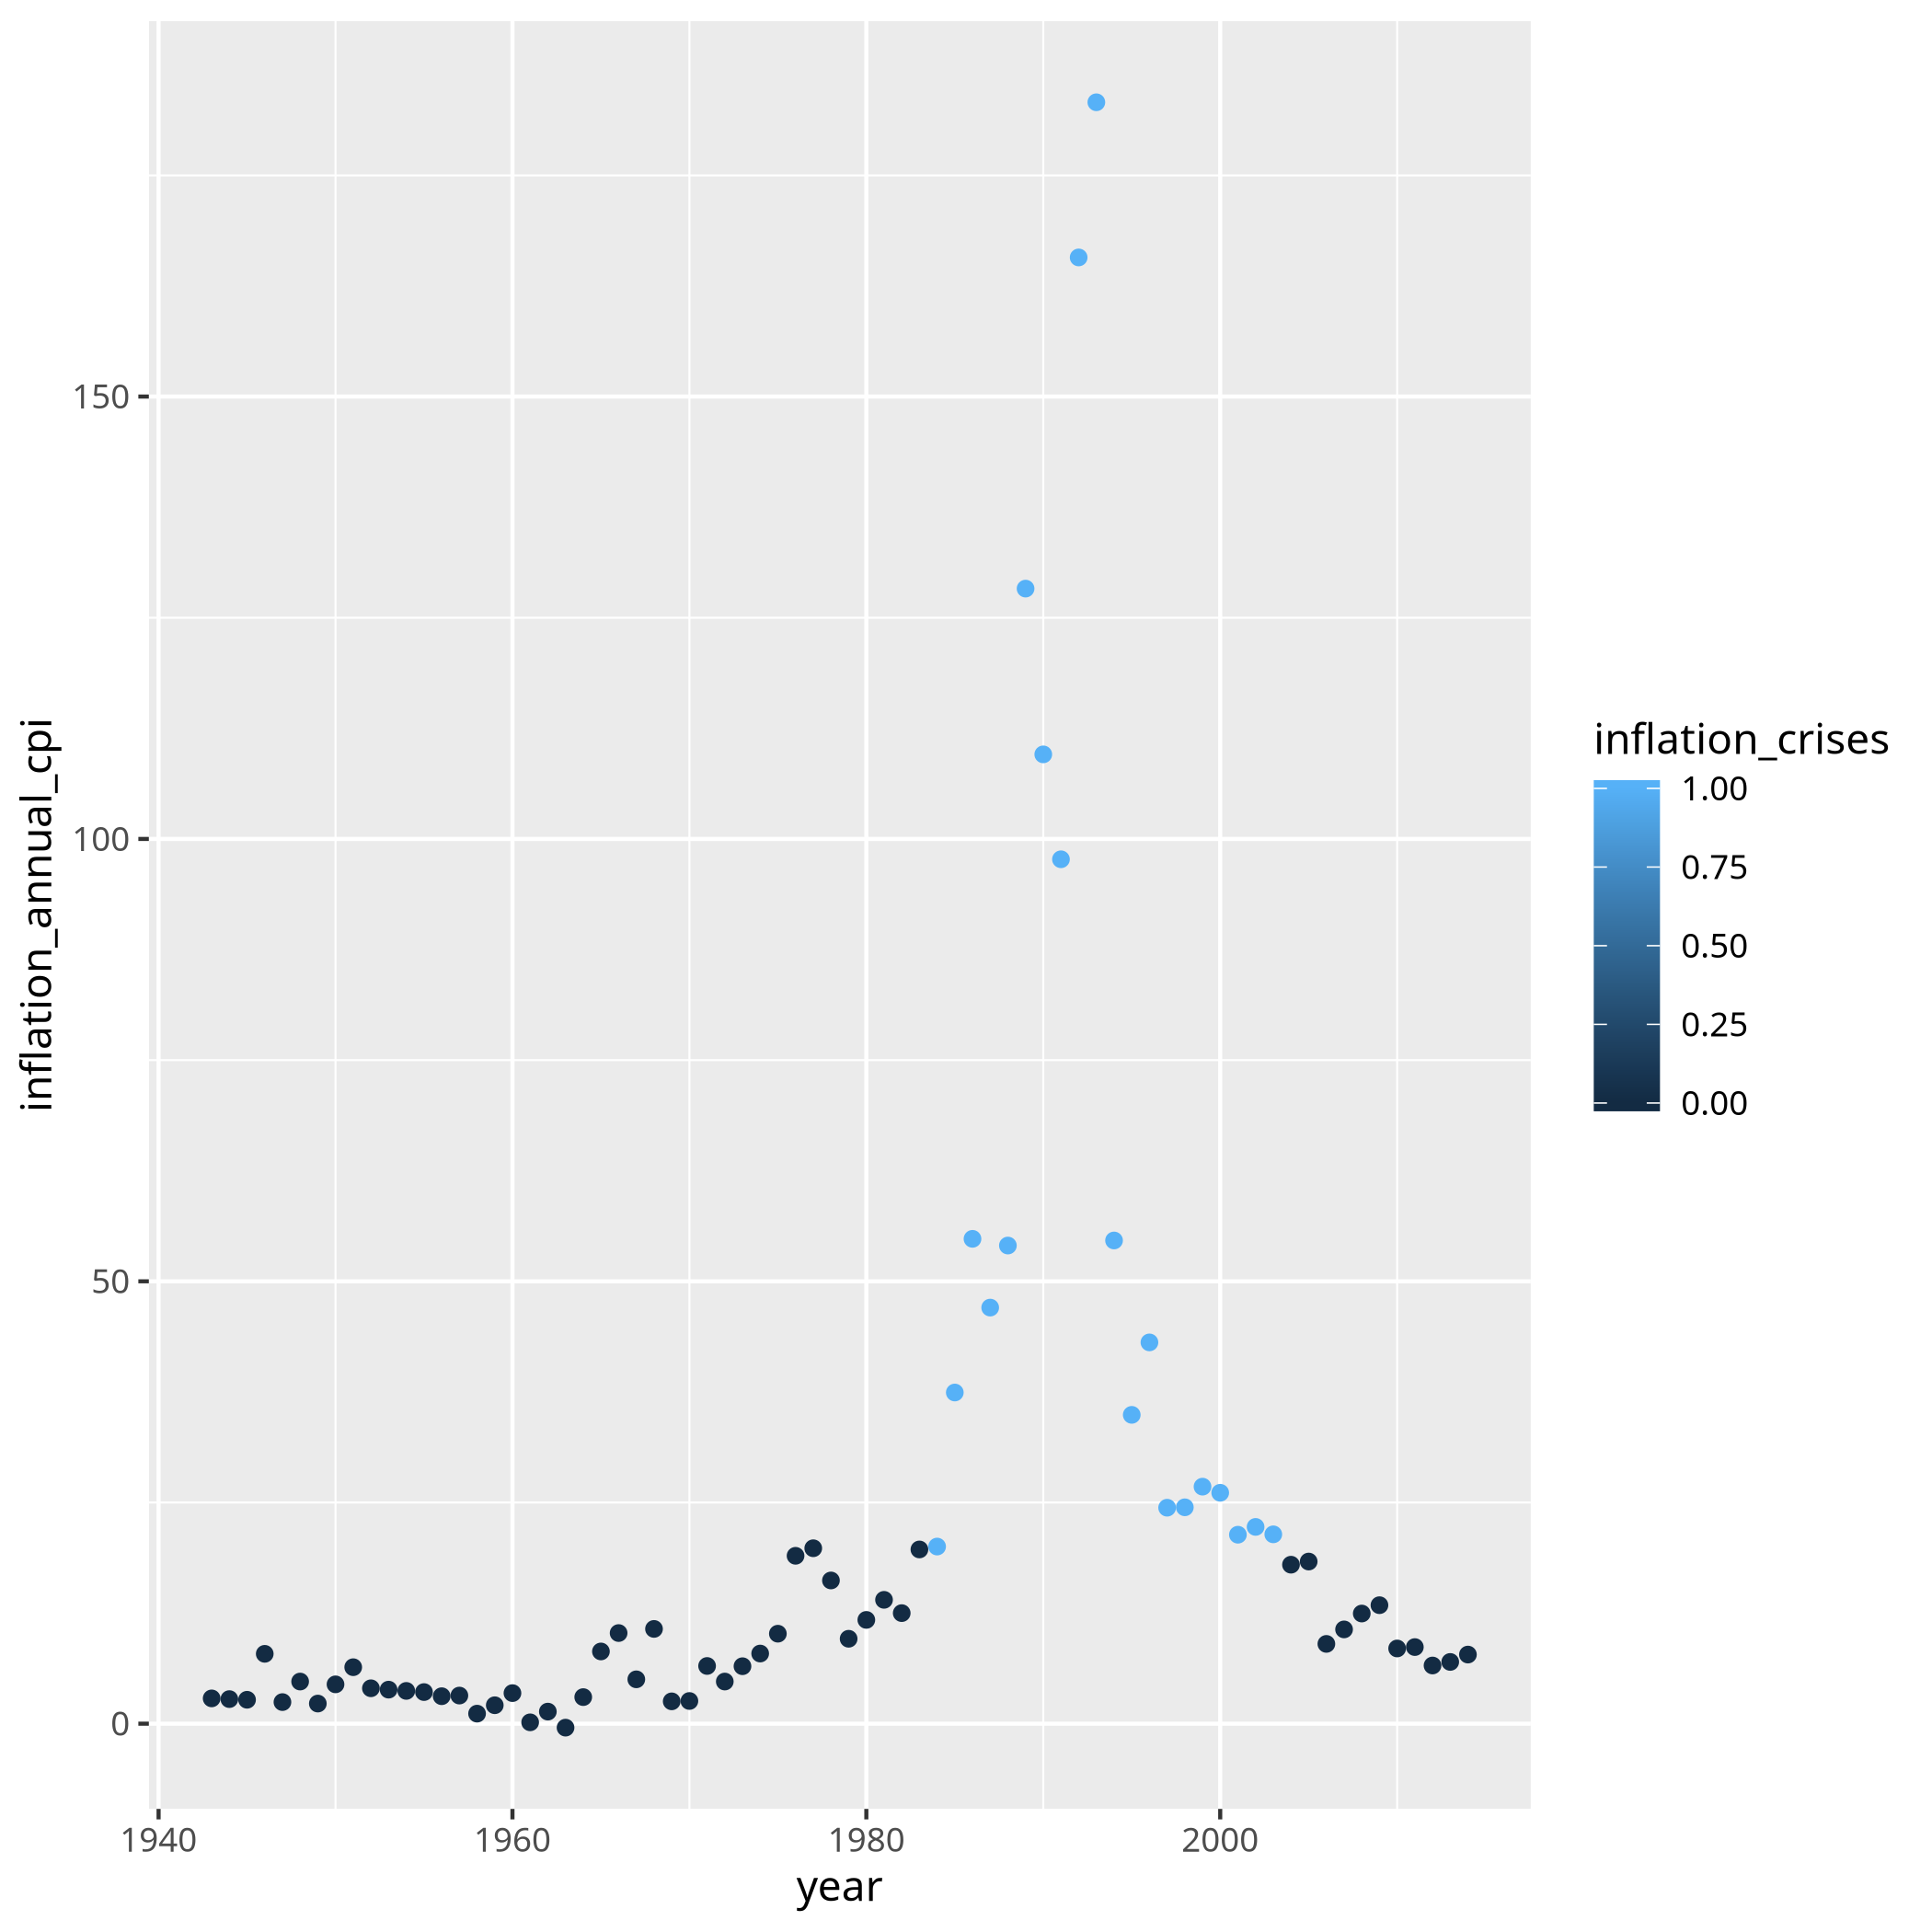
\includegraphics[scale=0.7]{plot3_zambia.png}
    \end{figure}

    \begin{figure}[h!]
        \caption{ USD Exchange rate in relation with a crisis in inflation in Zambia}
        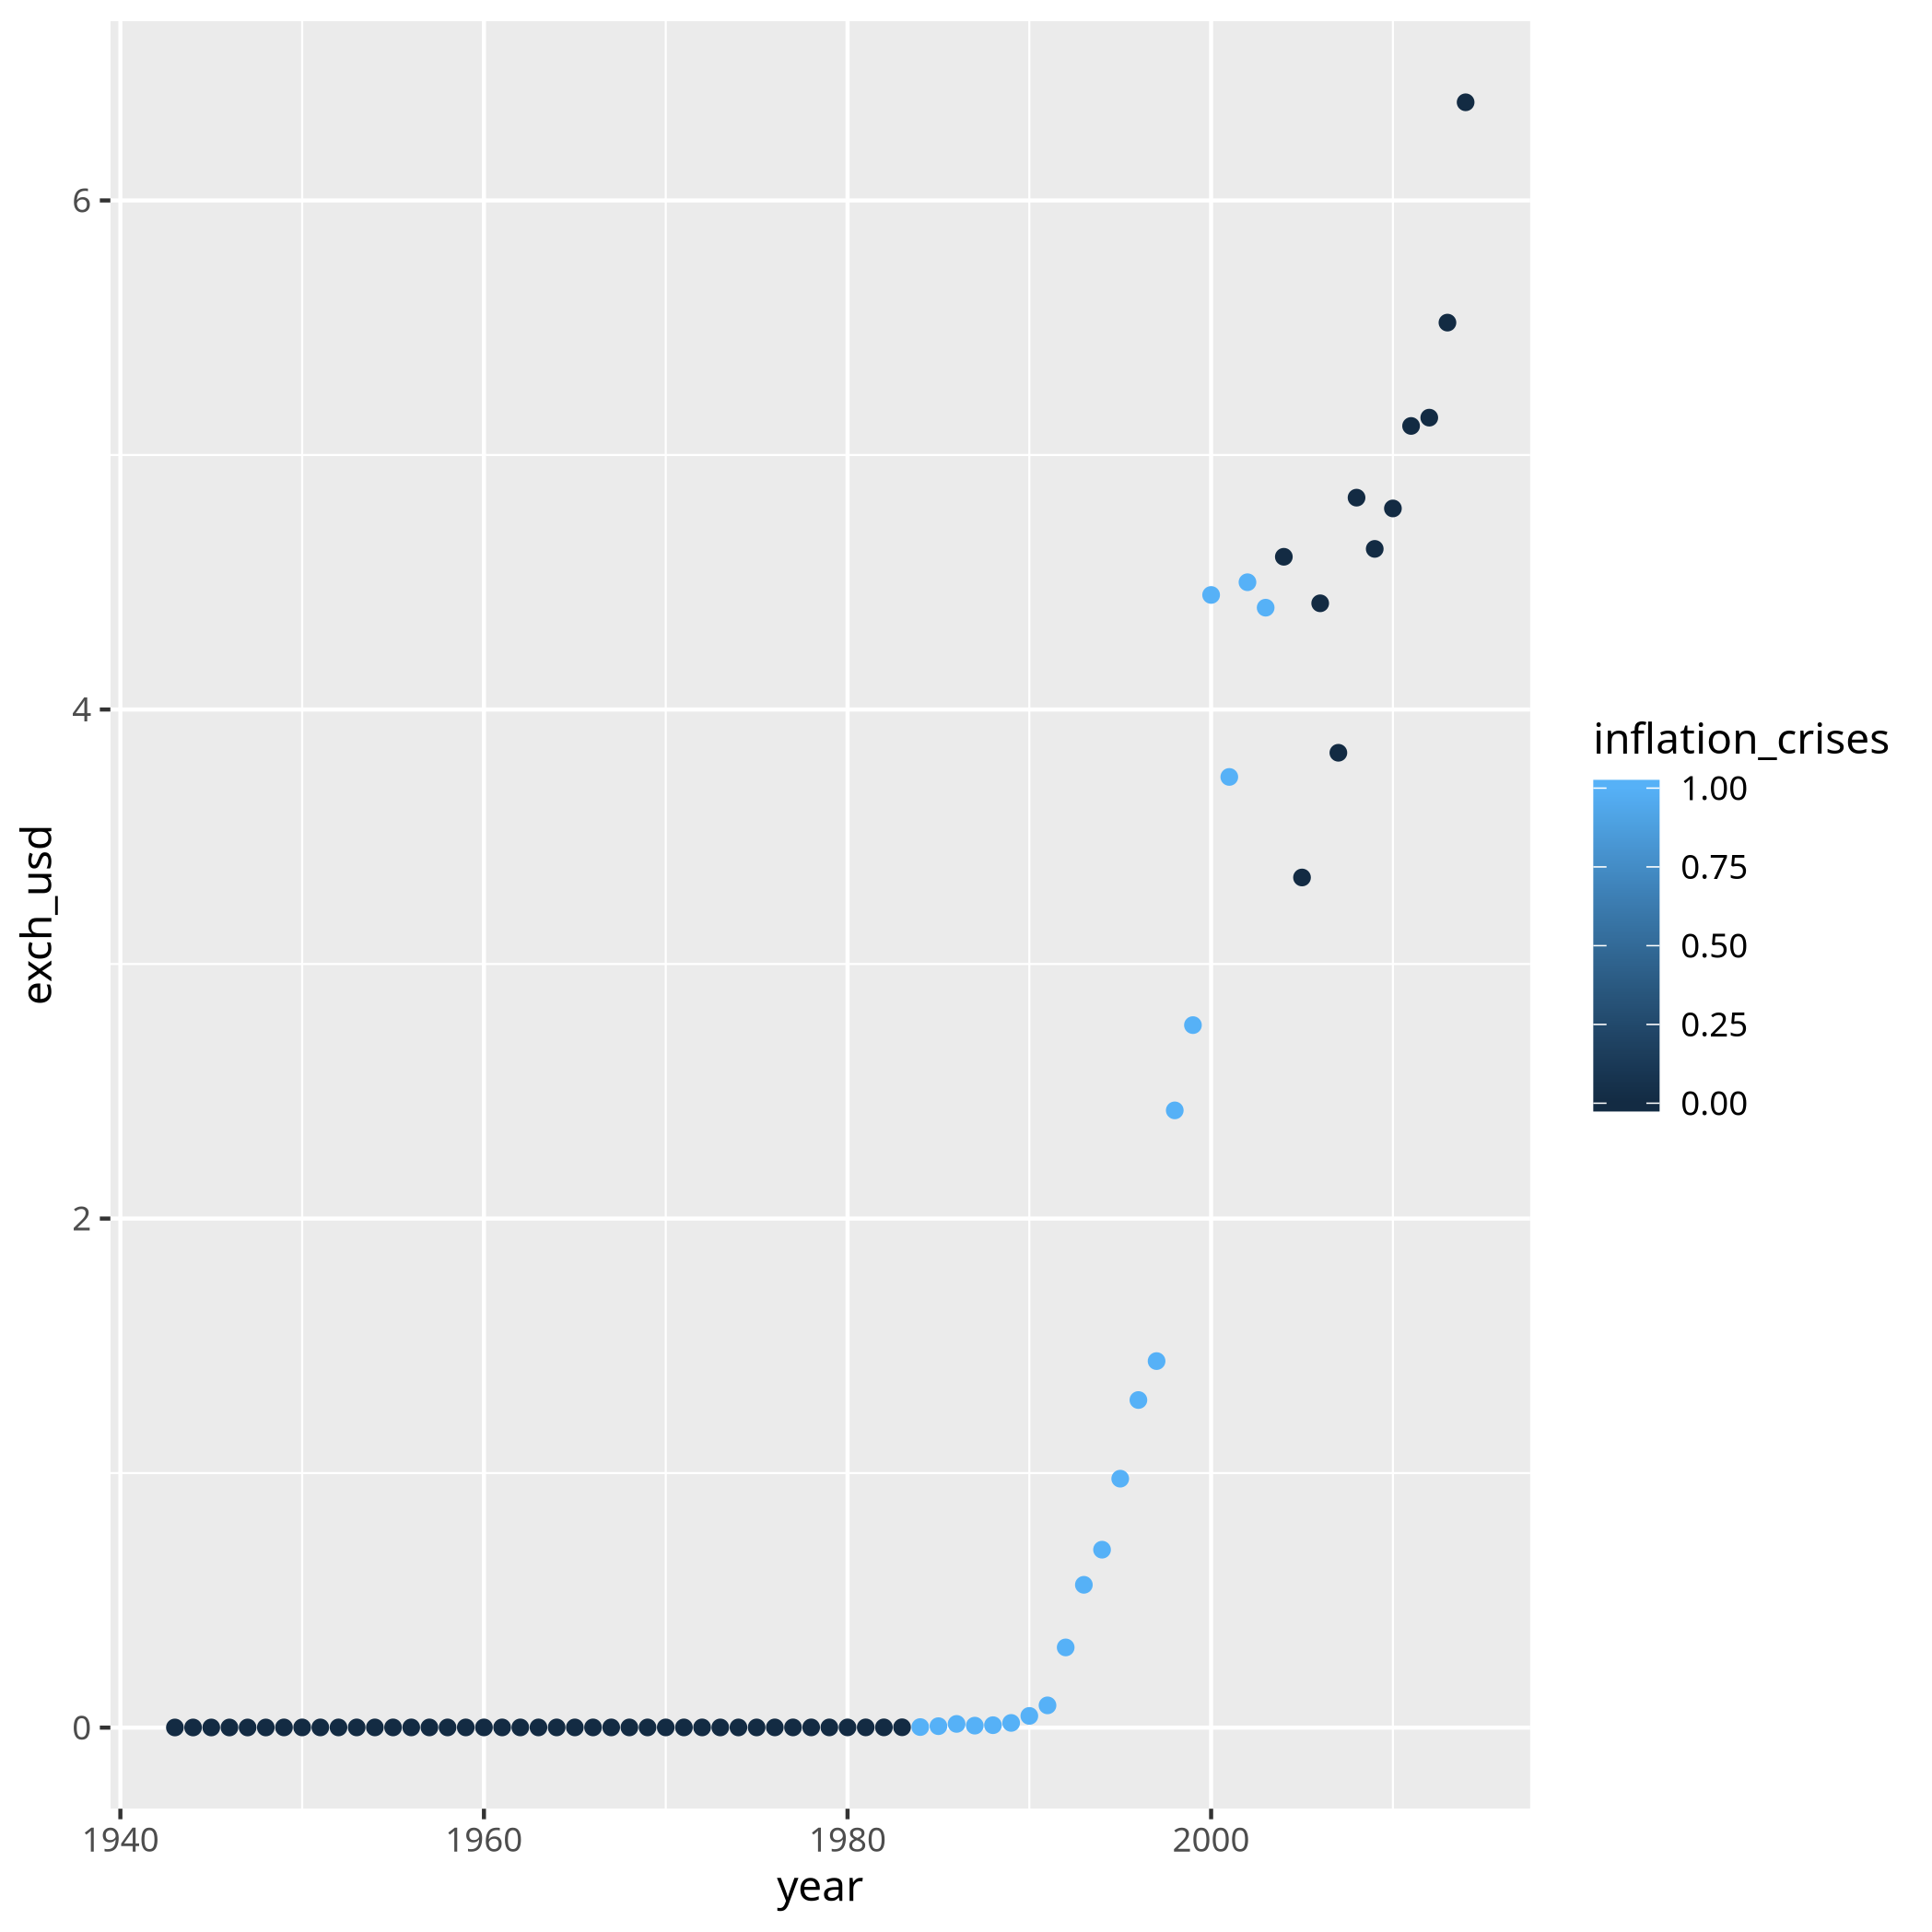
\includegraphics[scale=0.7]{plot3_exch_usd_zambia.png}
    \end{figure}
    \newpage

    By analyzing Figures 5 and 6, we can visualize that whenever there is an 
    \textbf{Inflation Crisis} in these countries, 
    that act as an example to a more general case in Africa, 
    hyperinflation occurs which leads to the result portrayed by Figure 6 
    where we can see Zambia's currency getting weaker as the Exchange Rate to the USD
    is getting higher.

    \newpage
    \section{ Independence }
    Most of the countries in this dataset were old European colonies with no \textbf{independence}
    until the 20th century. \textbf{Angola}, for example, was a \textbf{Portuguese} colony 
    and only got its independence on 1974 after 13 years of war. This greatly affected the
    countries' economies.

    
    \begin{figure}[h!]
        \caption{Independence of African Countries along the years and the relation with a banking crisis}
        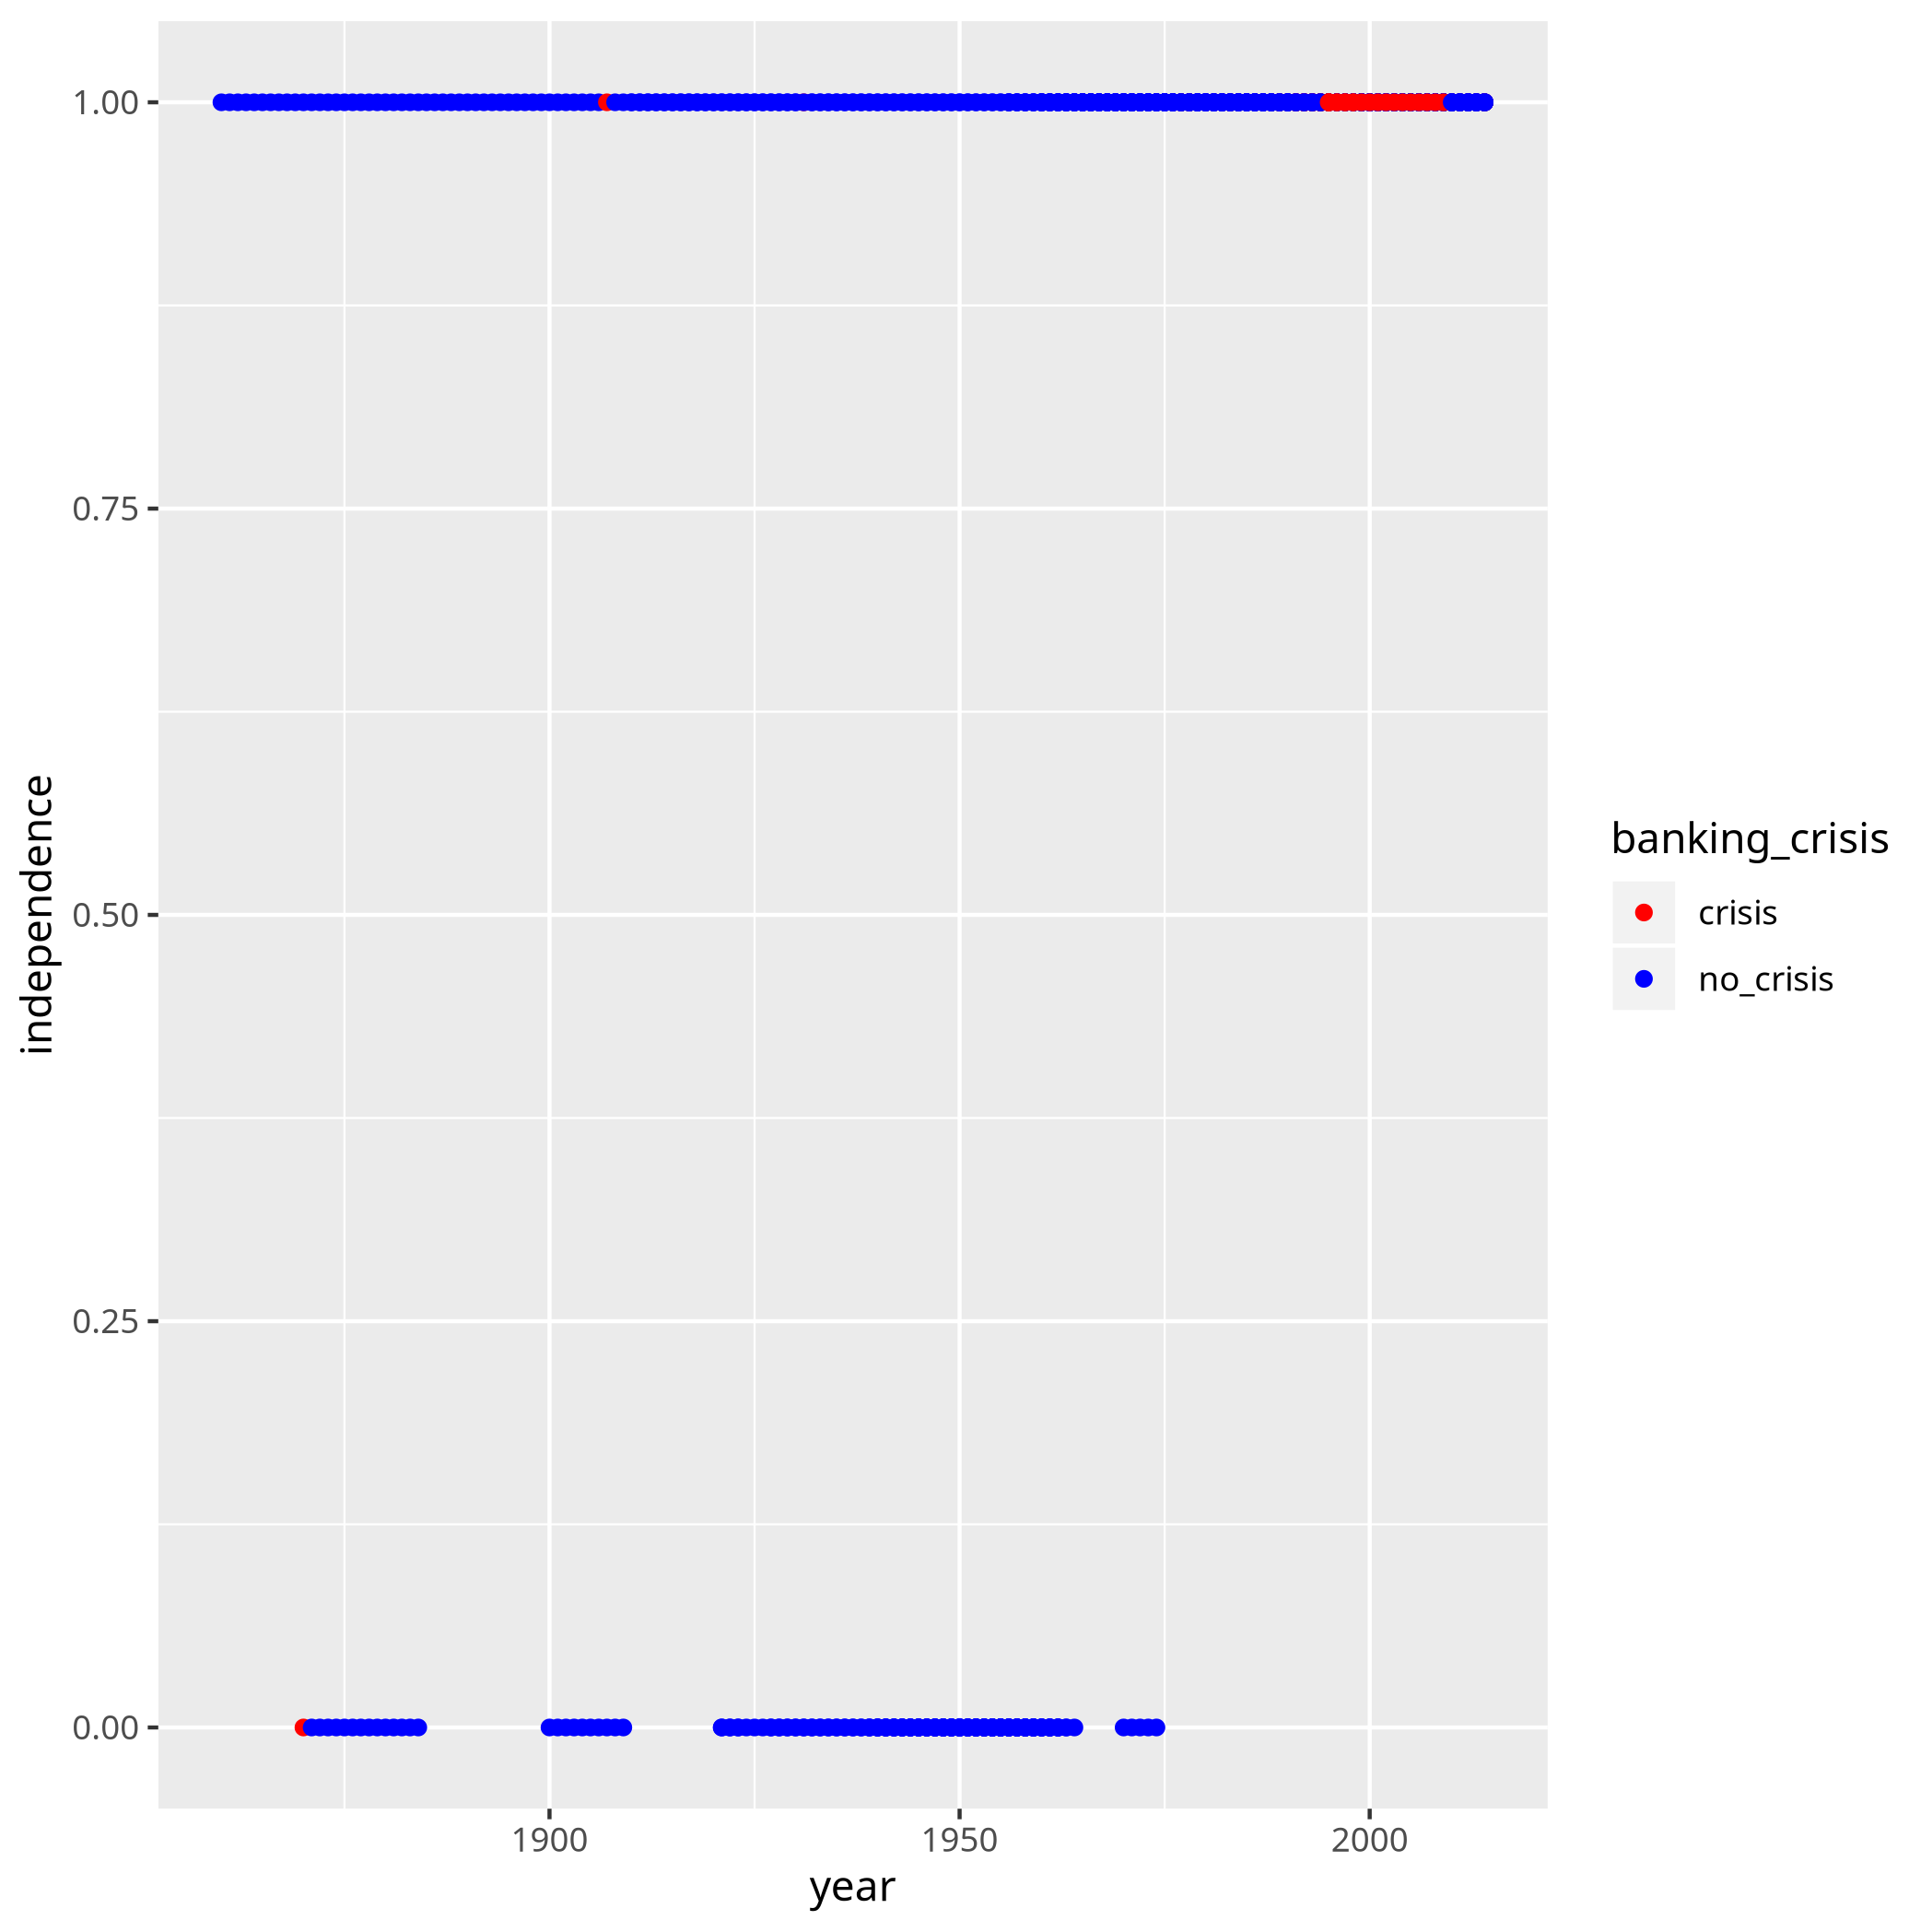
\includegraphics[scale=0.7]{plot5_general.png}
    \end{figure}
    \newpage
    \begin{figure}[h!]
        \caption{Independence of Nigeria along the years and the relation with a banking crisis}
        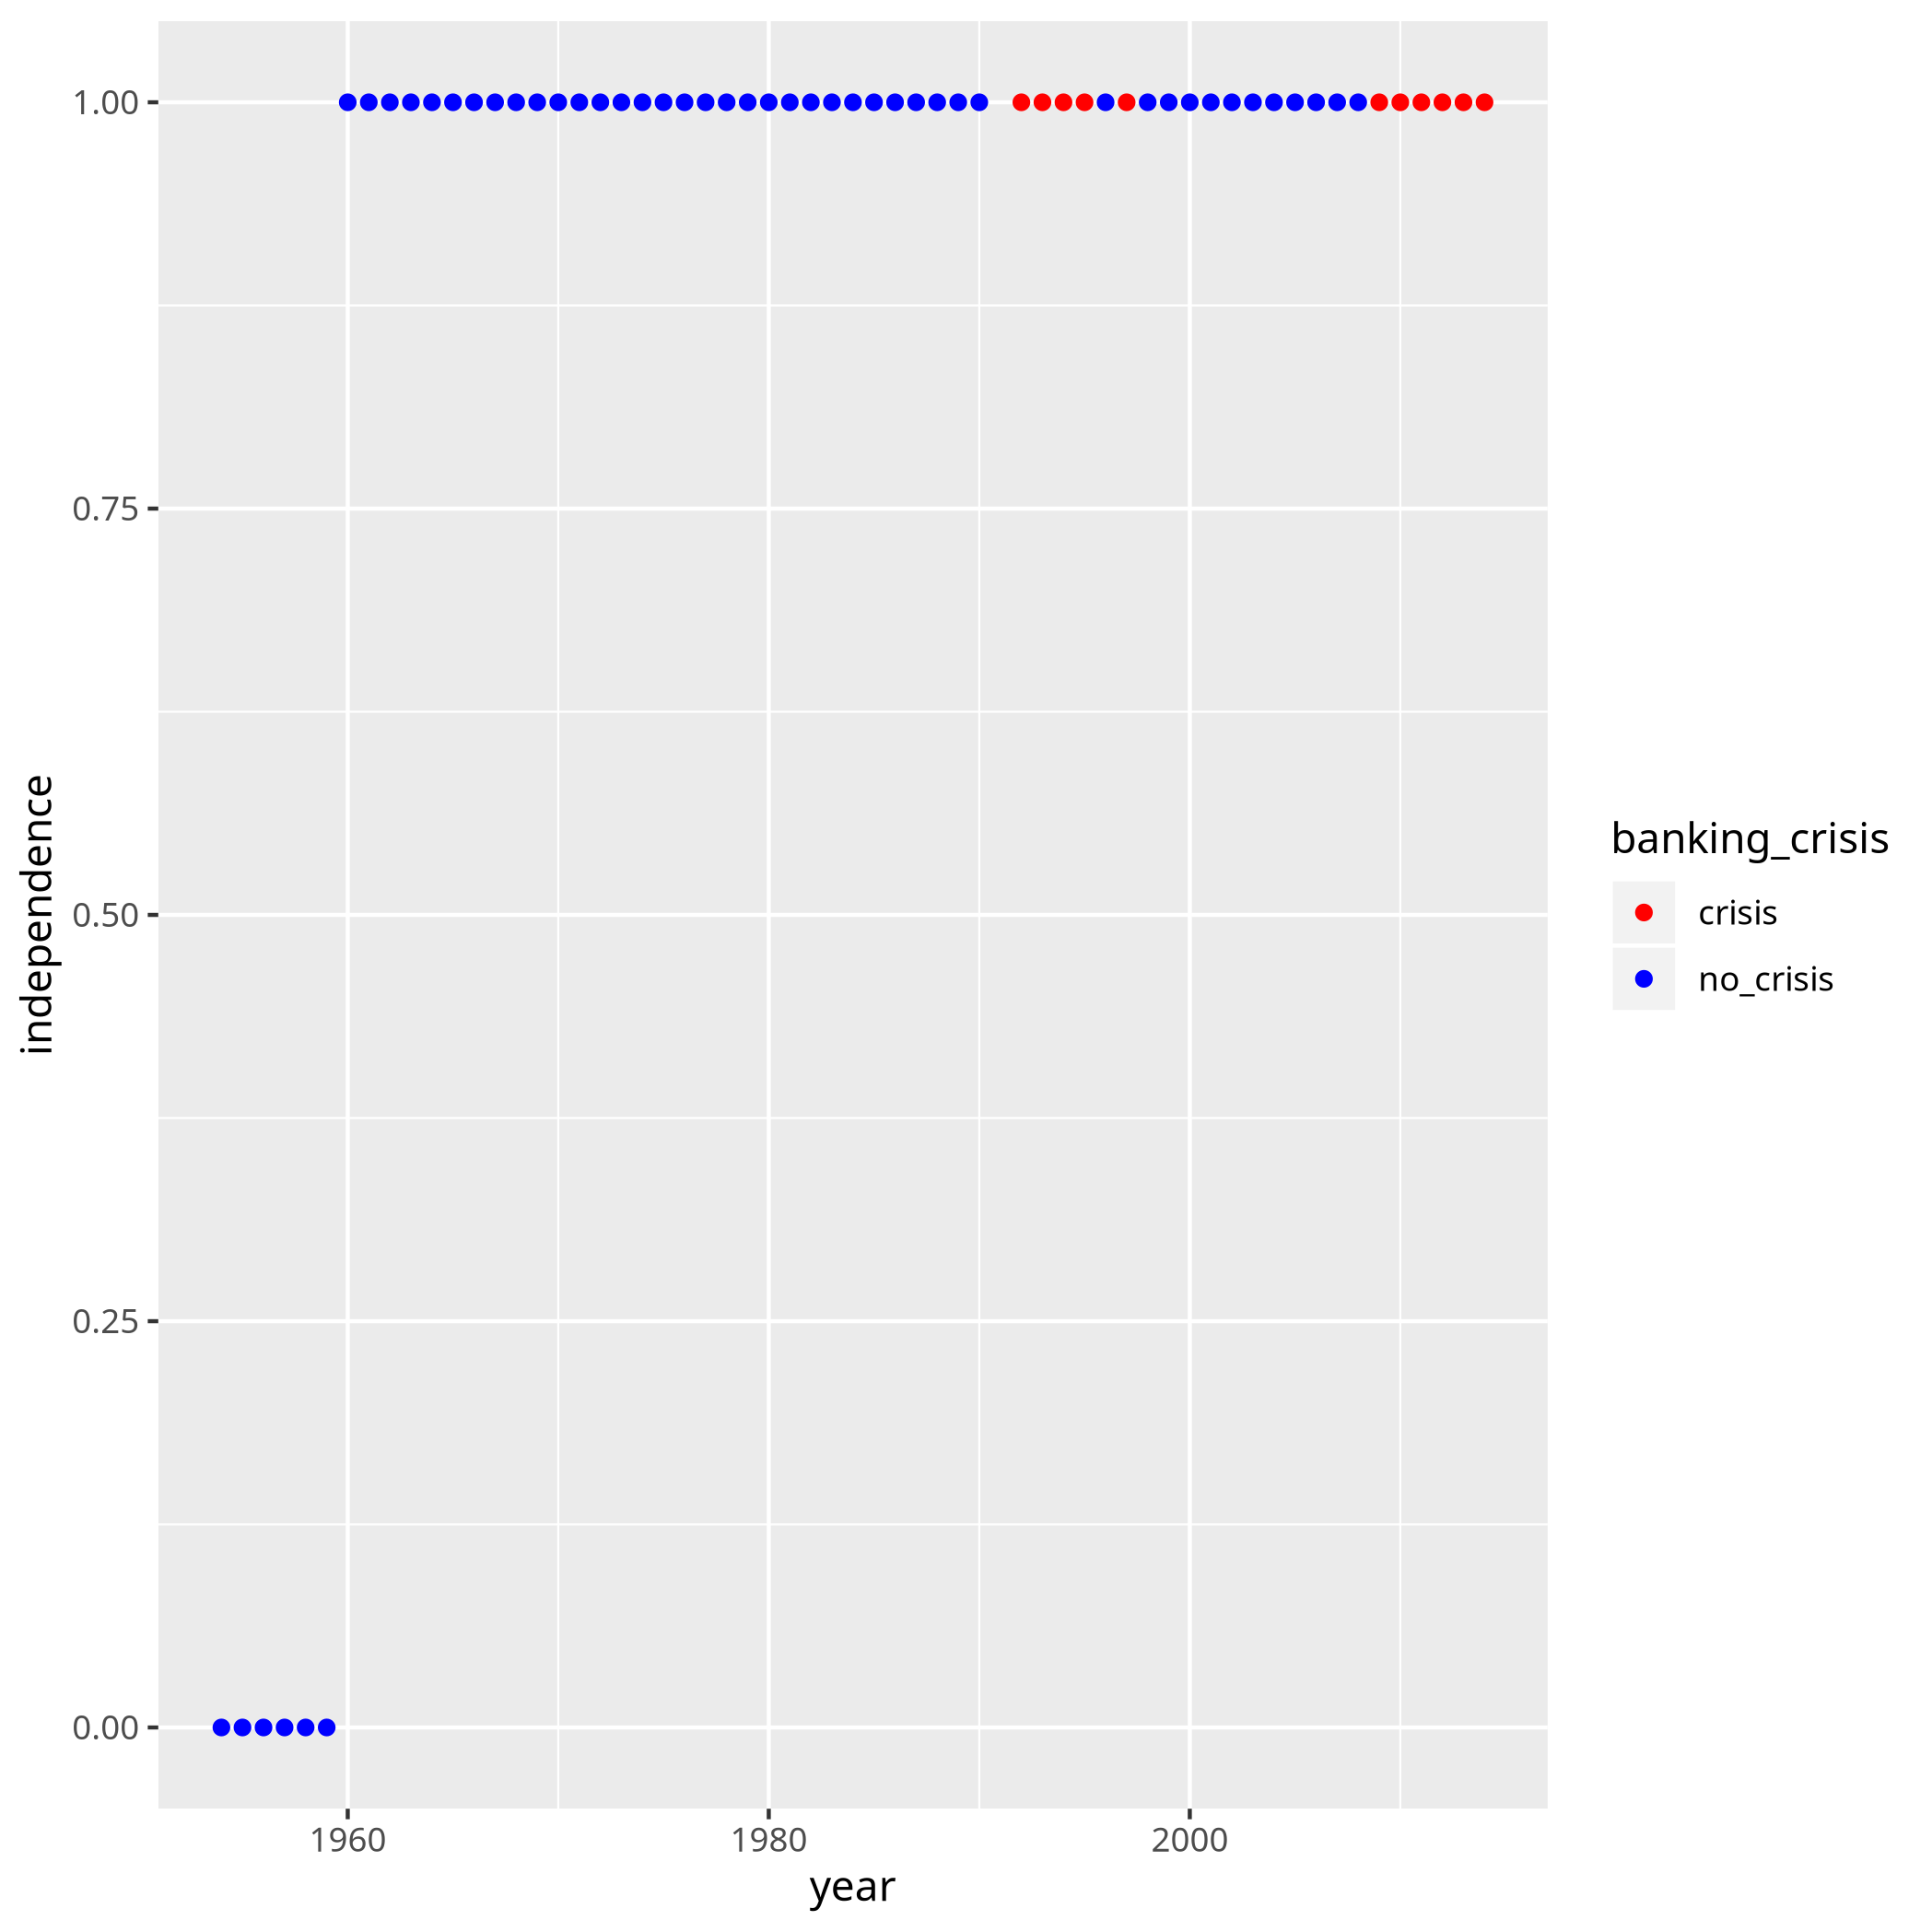
\includegraphics[scale=0.7]{plot5_nigeria.png}
    \end{figure}


    Both figures show that the banking crises only started after these countries obtained 
    \textbf{independence}. 
    Originally the sovereign states assured these provinces financial stability aided by 
    trade they provided in terms of resources. Of course this meant these countries were not 
    independent neither they were free, and so they each started their own battles to independence.
    However after that, generically, many of them ended up in years of civil war and 
    revolutions for government control, which ended up having devastating results to the countries' 
    economies and resulting in banking failures.
\end{document}